\documentclass[../TDON2_inter.tex]{subfiles}%

\begin{document}
\section[s]"3"{Interférences sur la cuve à ondes}

\enonce{%
	La figure ci-dessous représente une cuve à ondes éclairée en éclairage
	stroboscopique. Deux pointes distantes de a frappent la surface de l'eau de
	manière synchrone (même fréquence et phase à l'origine), générant deux ondes qui
	interfèrent. La figure est claire là où la surface de l'eau est convexe et
	foncée là où elle est concave. L'amplitude d'oscillation est plus faible là où
	la figure est moins contrastée.

	\begin{center}
		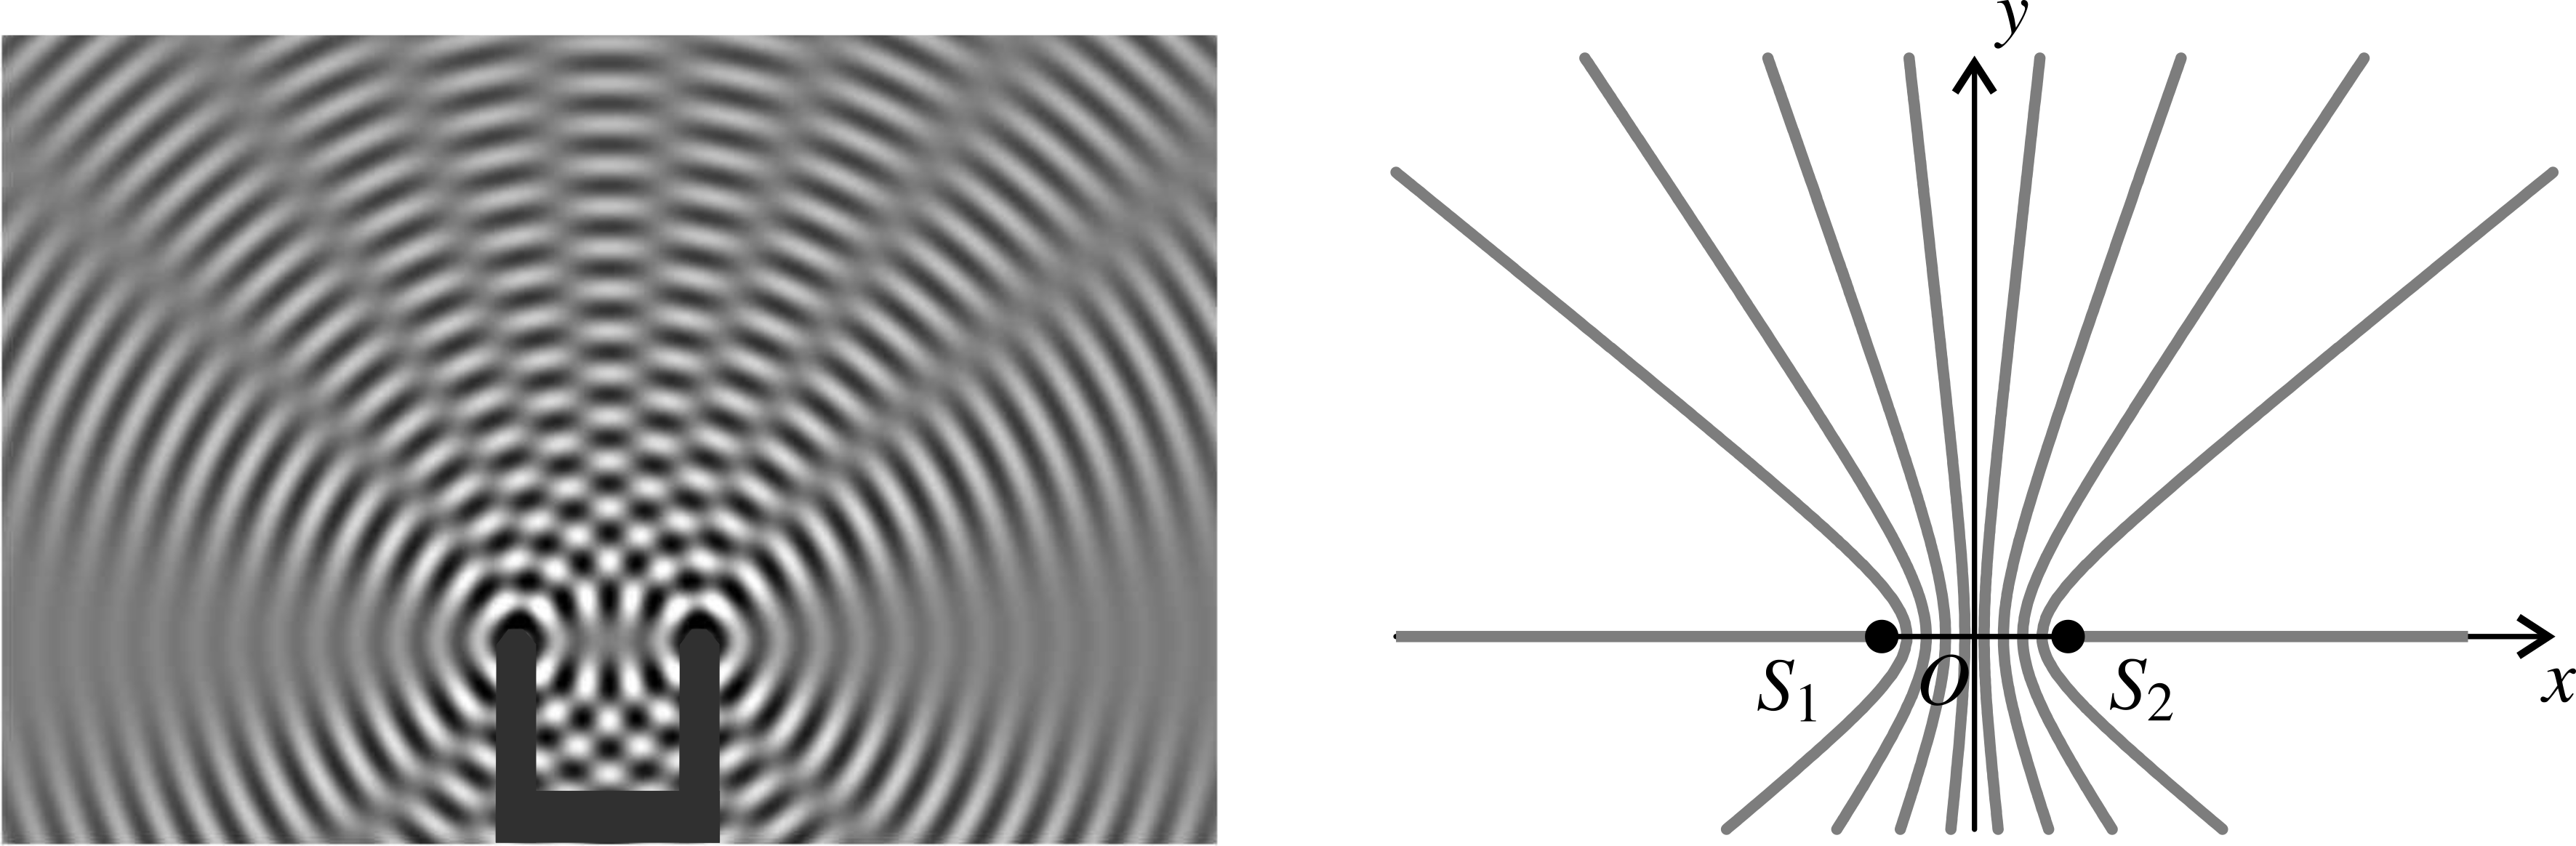
\includegraphics[width=.8\linewidth]{cuve_ondes-plain}
	\end{center}
}

\QR{%
	On suppose pour simplifier que des ondes sinusoïdales partent des deux
	points $S_1$ et $S_2$ où les pointes frappent la surface. En notant
	$\lambda$ la longueur d'onde, donner la condition pour que
	l'interférence en un point M situé aux distances $d_1$ et $d_2$
	respectivement de $S_1$ et $S_2$, soit destructrice. Cette condition
	fait intervenir un entier $m$.

}{%
	Par définition,
	\begin{gather*}
		\D\f_{1/2}(\Mr) = -k\D L_{1/2}(\Mr) = -k(d_1 - d_2) =
		\frac{2\pi}{\lambda}(d_2-d_1)
	\end{gather*}
	Et pour avoir des interférences destructives,
	\begin{gather*}
		\D\f_{1/2}(\Mr) = (2m+1)\pi
		\Lra
		\frac{2\cancel{\pi}}{\lambda}(d_2-d_1) = (2m+1)\cancel{\pi}
		\Lra
		\boxed{d_2-d_1 = \left(m+\frac{1}{2}\right)\lambda}
	\end{gather*}
}

\QR{%
	Pour chaque entier $m$ le lieu des points vérifiant cette condition
	est une courbe que l'on appelle dans la suite ligne de vibration
	minimale. Les lignes de vibration minimale sont représentées sur la
	figure de droite~: ce sont des hyperboles. Les parties $x < -a/2$ et $x
		> a/2$ de l'axe (O$x$) sont des lignes de vibration minimale. En déduire
	un renseignement sur $a/\lambda$.

}{%
	Avec ${\rm S_1S_2} = a$, on observe que tout l'axe $x > a/2$
	correspond à une ligne de vibration minimale, c'est-à-dire un endroit de
	l'espace où les interactions sont destructives, i.e. $d_2-d_1 =
		(m+1/2)\lambda$. Or, pour $x > a/2$, on a
	\begin{gather*}
		d_2 - d_1 = {\rm S_2M} - {\rm S_1M}
		= \cancel{\rm S_2M} - {\rm S_1S_2} + \cancel{\rm S_2M}
		\Lra
		\boxed{d_2 - d_1 = -a}
	\end{gather*}
	On en déduit donc
	\begin{gather*}
		\boxed{\abs{\frac{a}{\lambda}} = m+\frac{1}{2}}
	\end{gather*}
	c'est-à-dire que $a/\lambda$ est un demi-entier (1/2, 3/2, 5/2…). Le
	résultat est le même en raisonnant sur $x < -a/2$.
}

\QR{%
	Sur le segment S$_1$S$_2$, quel est l'intervalle de variation de $d_2
		- d_1$~? Déduire de la figure la valeur de $a/\lambda$.
}{%
	Entre $\rm S_1$ et $\rm S_2$, on prend 3 cas extrêmes pour déterminer
	l'amplitude de $d_2 - d_1$~:
	\begin{itemize}
		\item En $\rm S_1$, $d_2 = -a$ et $d_1 = 0$, donc
		      \[d_2 - d_1 = -a\]
		\item En O, $d_2 = -a/2$ et $d_1 = a/2$, donc
		      \[d_2 - d_1 = 0\]
		\item En $\rm S_2$, $d_2 = 0$ et $d_1 = a$, donc
		      \[d_2 - d_1 = -a\]
	\end{itemize}
	Ainsi,
	\begin{gather*}
		\boxed{-a \leqslant d_2 - d_1 \leqslant a}
	\end{gather*}
	Or, entre $\rm S_1S_2$ on observe plusieurs vibrations minimales,
	donnant chacune $d_2 - d_1 = (m+\frac{1}{2})\lambda$. On en compte 8
	entre $\rm S_1S_2$, correspondant chacune à un ordre d'interférence $m$.
	À partir de O et vers les $x$ croissants, on a la première vibration
	minimale pour $m=0$, la deuxième pour $m=1$, la troisième pour $m=2$ et
	la dernière pour $m=3$~; on a de même par symétrie vers les $x$
	décroissants. Ainsi, \textbf{l'ordre d'interférence obtenu le plus grand
		est $m=3$}, et \textbf{on n'a pas l'ordre d'interférence $m=4$} sinon on
	aurait une parabole en plus de chaque côté. Ainsi,
	\begin{gather*}
		\left(3+\frac{1}{2}\right)\lambda
		< a \leqslant
		\left(4+\frac{1}{2}\right)\lambda
	\end{gather*}
	puisqu'on observe qu'il reste une distance sur $\rm S_1S_2$ après
	l'ordre 3 avant d'atteindre S$_2$ et que si $a$ dépasse $(4+1/2)\lambda$
	on verrait la parabole correspondant à l'ordre 4. Comme on a déterminé à
	la question précédente que $\frac{a}{\lambda} = m + \frac{1}{2}$, avec
	cette étude on a $3 < m \leqslant 4$ avec $m \in \Nb$, autrement dit
	\fbox{$m = 4$}, soit
	\[\boxed{\frac{a}{\lambda} = \frac{9}{2}}\]
}

\QR{%
	Expliquer pourquoi l'image est bien contrastée au voisinage de l'axe
	(O$y$).
}{%
	Le contraste correspond à une grande différence entre les valeurs
	maximales et minimales. Or, sur (O$y$) on a $d_2 = d_1$ donc $d_2-d_1 =
		0$, c'est-à-dire que les ondes sont en phase et les interférences
	constructives, donc l'amplitude est maximale et le contraste est élevé.
}
\end{document}
